%TITLE, AUTHOR, DATE
\documentclass[18pt, a4paper]{extarticle} %14 pt indicates the font size of the prepared document
\usepackage[margin=1in]{geometry}
\usepackage[utf8]{inputenc}
\usepackage{multicol}
\usepackage{multirow}
\usepackage{color}
\usepackage{enumerate}
\usepackage{amsmath}
\usepackage{graphicx}
\usepackage{fontsize}
\changefontsize[18pt]{11pt}

\title{CSE 300: Online Assignment}
\author{Md Shamsuzzoha Bayzid, Mahjabin Nahar, Md Shariful Islam Bhuyan,\\
	and Md Saidur Rahman}
\date{April 2021}

\begin{document}
	\maketitle
	
	 \section{Introduction}
	 This assignment has been designed to assess the preparation of the students in writing
	 scientific articles using \LaTeX. This assignment covers a variety of components that are
	 commonly used in scientific manuscripts.
	
	 \subsection{Figures}
	 We intend to put Figure 1 at the top of a page.
	 
	 \subsection{Tables}
	 We wish to place Table 1 right here.
	 
	 \begin{table}[h]
	 	\centering
	 	\caption{\textbf{Optimization scores for Method-1 and Method-2 on different datasets covering various model conditions.} We show average scores of two optimization criteria for various model conditions.}

	 	\vspace{10mm}
	 	\begin{tabular}{|c|c|c|c|c|c|}
	 		\hline
	 		Dataset & Model & \multicolumn{2}{|c|}{Optimization Score 1} & \multicolumn{2}{|c|}{Optimization Score 2}\\
	 		\cline{3-6} % hline from col 3 to col6
	 		& condition & Method-1 & Method-2 & Method-1 & Method-2 \\
	 		\hline
	 		\hline
	 		
	 		\multirow{4}{*}{D1} & $M_1$ & 7,425.55 & 770.00 & 929.55 & 10 \\
	 		& $M_2$ & 7,657.00 & 9,179.00 & 716.15 & 20 \\
	 		& $M_3$ & 54.00 & 9,007.15 & 3,759.00 & 30 \\
	 		& $M_4$ & 74.00 & 5567.15 & 99.00 & 25 \\
	 		\hline
	 		
	 		\multirow{3}{*}{Dd2} & $M_1$ & 34.00 & 273.00 & 321.60 & 34 \\
	 		& $M_2$ & 357.00 & 79.60 & 16.00 & 11 \\
	 		& $M_3$ & 657.00 & 179.60 & 716.00 & 19 \\
	 		\hline
	 		
	 	\end{tabular}
	 \end{table}
	 \newpage
	 
	 %% add a pdf file/figure
	 
	 \begin{figure}[h!]
	 	%...
	 	\centering
	 	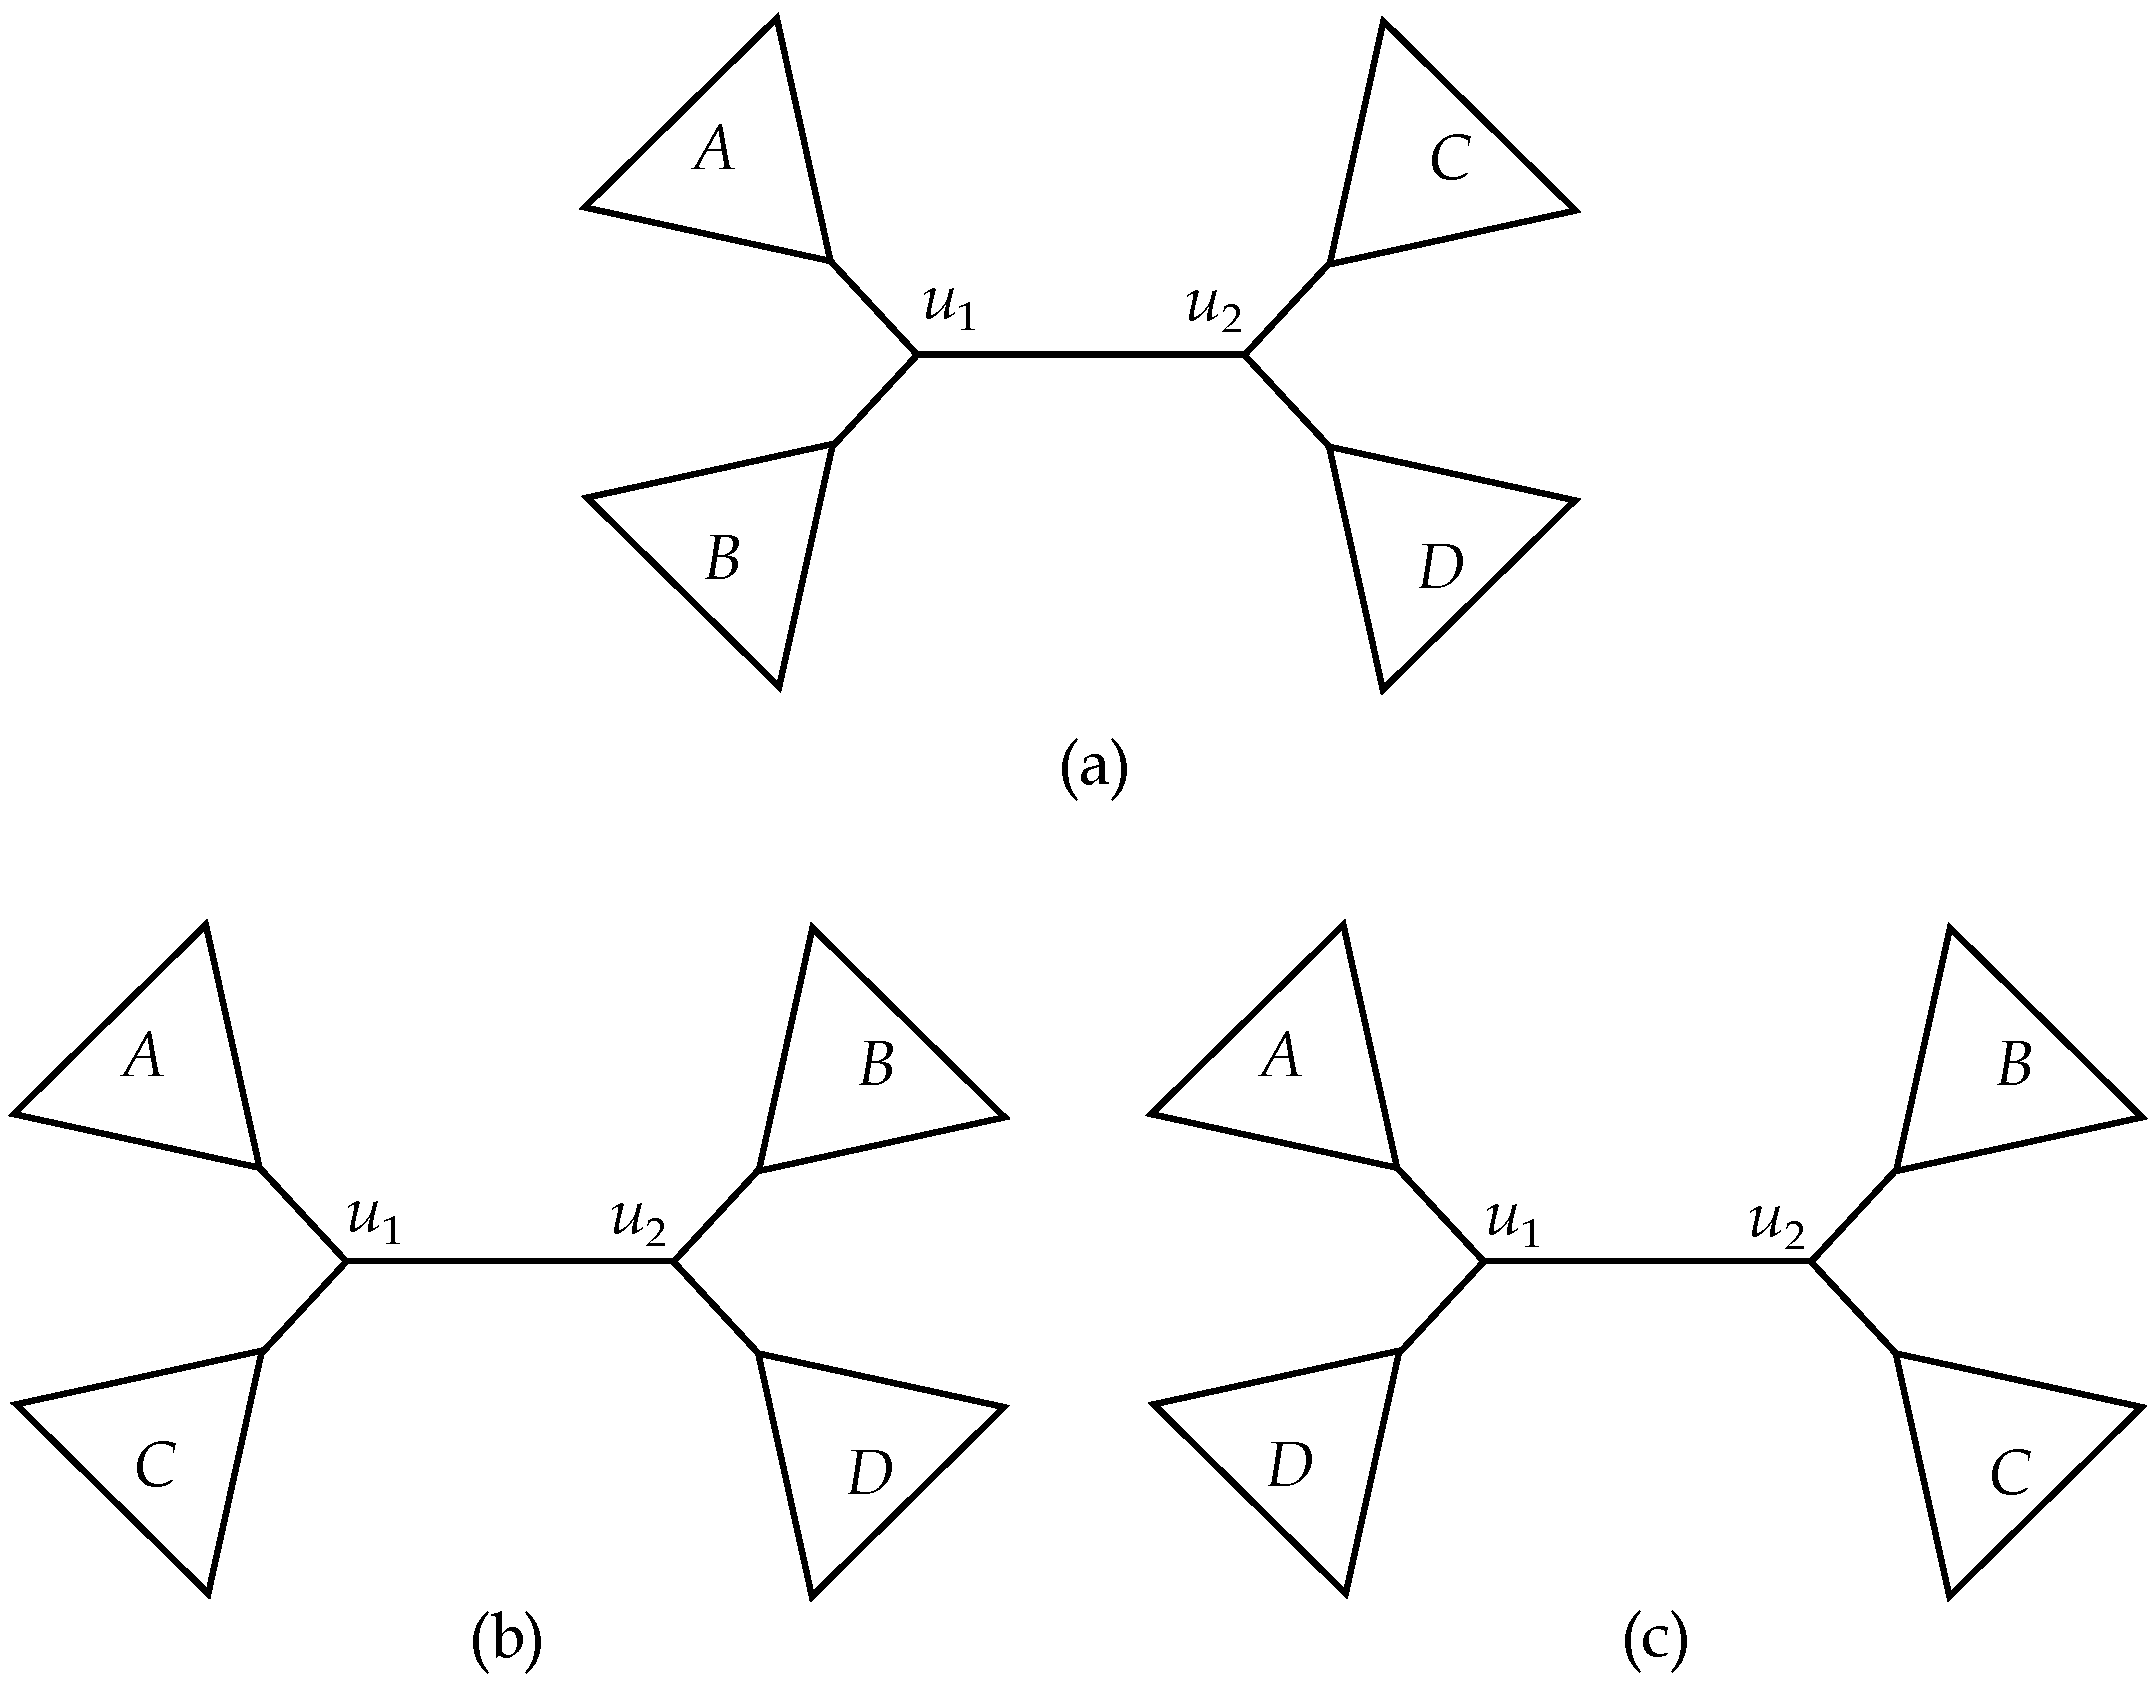
\includegraphics[scale=0.3]{Figure3.pdf}
	 	\caption{\textbf{Nearest Neighbor Interchange (NNI) move on an internal edge.} (a)
	 		A species tree ST, and (b)-(c) the neighbors of ST resulting from one NNI move on edge
	 		e = (u1, u2). A, B, C, and D are the sets of taxa in the four subtrees around edge e.}
	 \end{figure}
 
 	\subsection{Equations}
 	Let $n1|n2|n3$ be a tripartition defined on an internal node $u$ of a binary tree $T$. The number of tripartitions mapped to $u$ is given by Eqn. 1.
	 
	\begin{equation}
		\mathcal{N}\mathcal{Q} (n_1,n_2,n_3)=\binom{n_1}{2}\binom{n_2}{1}\binom{n_3}{1}+\binom{n_2}{2}\binom{n_1}{1}\binom{n_3}{1}+\binom{n_1}{2}\binom{n_1}{1}\binom{n_2}{1}
	\end{equation}

	\section{Conclusion}
	The major objectives of this assignment are listed below (please do not ignore the font sizes).
	
	
	\begin{enumerate}
		\item \Large{To assess the ability of the students in preparing manuscripts in \LaTeX.}
		\item[\Large{2.}] \large{To see if the students have adequately practiced different aspects of
writing in \LaTeX.}
		\item[\large{3.}] \normalsize{To see if the students can add various basic components (e.g., tables, figures, equations) to a \LaTeX   
			manuscript.}
		
		\newpage
		
		\item[4.] To see if the students can leverage the available materials (both offline and online) to do
		something which has not explicitly been taught in the class.
		
	\end{enumerate}
	
	 
	 
\end{document}
